%% LyX 2.1.4 created this file.  For more info, see http://www.lyx.org/.
%% Do not edit unless you really know what you are doing.
\documentclass[12pt,french]{article}
\usepackage[T1]{fontenc}
\usepackage[utf8]{inputenc}
\usepackage[a4paper]{geometry}
\geometry{verbose,tmargin=3cm,bmargin=3cm,lmargin=3cm,rmargin=3cm}
\setlength{\parskip}{\medskipamount}
\setlength{\parindent}{0pt}
\usepackage{babel}
\makeatletter
\addto\extrasfrench{%
   \providecommand{\og}{\leavevmode\flqq~}%
   \providecommand{\fg}{\ifdim\lastskip>\z@\unskip\fi~\frqq}%
}
%  make4ht -d temp/ -u horoch_juin2016.tex -c horoch_juin2016 "html,1"
\makeatother
\usepackage{url}
\usepackage{graphicx}
\usepackage{setspace}
\usepackage{esint}
\onehalfspacing
\usepackage[unicode=true,pdfusetitle,
 bookmarks=true,bookmarksnumbered=false,bookmarksopen=false,
 breaklinks=false,pdfborder={0 0 1},backref=false,colorlinks=false]
 {hyperref}

\makeatletter

%%%%%%%%%%%%%%%%%%%%%%%%%%%%%% LyX specific LaTeX commands.
%% Because html converters don't know tabularnewline
\providecommand{\tabularnewline}{\\}

%%%%%%%%%%%%%%%%%%%%%%%%%%%%%% User specified LaTeX commands.
\usepackage{tikz}
\tikzstyle{every picture}+=[remember picture]
\usetikzlibrary{decorations.pathmorphing}
\tikzset { domaine/.style 2 args={domain=#1:#2} }

\makeatother

\begin{document}

\title{Projet HOROCH: T131 Rapport d’étude et d’évaluation des performances sur la parallélisassions hybride}
\date{Juin 2016}
\author{Philippe Helluy, Bruno Weber}

\maketitle

\section{Principes du parallélisme par tâches}


\subsection{Généralités}

Actuellement, la plupart des codes de calculs intensifs exploitant
les supercalculateurs reposent sur les technologies OpenMP et MPI.
OpenMP est utilisé pour attaquer le parallélisme à l'intérieur d'un
nœud de calcul, qui est généralement constitué de plusieurs CPU multicœurs
partageant une mémoire commune. MPI permet d'échanger des données
entre les nœuds de calcul.

Ce découpage repose sur l'hypothèse de calculs très uniformes dont
il est possible de connaître à l'avance le coût élémentaire. Il faut
aussi que les échanges de données soient relativement faibles comparés
au volume des calculs. Par ailleurs, la stratégie est efficace pour
une résolution qui n'utilise pas de marche en temps locale, qui repose
sur des maillages relativement uniformes et des calculs qui ne nécessitent
pas trop de traitements particuliers (comme par exemple des calculs
ou des transferts de données auxiliaires).

La conception actuelle de Teta repose sur cette hypothèse. La seule
différence avec l'approche OpenMP/MPI est que dans Teta, le parallélisme
à l'intérieur du noeud est réalisé au moyen d'OpenCL afin de pouvoir
utiliser n'importe quel type d'accélérateurs, coeurs de CPU aussi
bien que des GPU.

Actuellement, de nombreux outils ont été développés par les chercheurs
en informatique pour rendre la parallélisation de codes plus facile.
Il existe des logiciels qui permettent par exemple de produire
automatiquement du code OpenMP à partir d'un code C séquentiel. Il existe
aussi des outils, appelés ``supports d\textquoteright exécution'' ou
``runtime'' qui permettent de soumettre des tâches de calcul à une file
d'attente. C'est le runtime qui se charge alors de distribuer en parallèle
les tâches sur les accélérateurs en fonction des dépendances entre les
tâches. Dans les systèmes les mieux conçus, c'est le runtime qui calcule
les dépendances entre les tâches.

Le but de cette partie du projet a été d'évaluer divers types outils
automatiques afin de mettre en œuvre une parallélisation hybride.


\subsection{Outils existants}

Dans ce paragraphe, on liste quelques outils automatiques. Il est
impossible d\textquoteright être exhaustif, car c'est un domaine où
les développements sont très actifs à la fois en terme de recherche
et de développement technologique.


\subsubsection{OpenMP}

OpenMP est un standard qui est aujourd'hui très répandu dans le domaine
du HPC. Il est intéressant pour le développeur, car il permet d'introduire
du parallélisme de manière incrémentale dans un code séquentiel déjà
existant au moyen de ``directives'': il suffit d'annoter le code
là où il doit être parallélisé. Si le compilateur n'est pas compatible
avec OpenMP, les annotations sont tout simplement ignorées, car elles
sont considérées comme de simples commentaires. La méthode la plus
classique consiste à vectoriser les boucles dont chaque terme peut-être
calculé indépendamment des autres. Il existe aussi des directives
pour calculer des réductions parallèles (somme des termes d'un vecteur,
par exemple). Depuis les normes 3 et 4 d'OpenMP il est également possible
de décrire des tâches et leurs dépendances. Depuis OpenMP 4 il est
possible de planifier des tâches sur des accélérateurs de type GPU.
HMPP et OpenACC sont d'autres outils basés sur des directives qui
permettent d'accéder à des GPU.

Avec OpenMP il est en général assez facile d'accélérer un code d'un
facteur deux à dix. Mais au-delà de dix cœurs la gestion des accès
mémoire devient très importante. Il faut tenir compte de ces accès
et une réorganisation du code devient nécessaire. Par ailleurs la
coexistence de deux logiques différentes, séquentielle et parallèle
au sein d'un même programme rend rapidement le code source difficile
à lire. Comme pour tout développement de code parallèle, le débogage
est délicat, car c'est au programmeur de gérer les conflits d'accès
aux données.

En conclusion, OpenMP semble offrir le standard le plus stable à moyenne
et longue échéance pour décrire du parallélisme. Mais modifier incrémentalement
un code séquentiel permet rarement une accélération optimale. De toute
façon, le parallélisme doit être intégré à la conception initiale
du logiciel. Selon la littérature que nous avons pu consulter, la
parallélisation par directive permet d'accélérer d'un facteur de l'ordre
de 4 un code en déportant une partie des calculs sur GPU. Mais le
facteur limitant est imposé par les transferts CPU/GPU et les accès
mémoire.

Lorsque l'on vise des performances très élevées, il n'est donc
pas tellement plus efficace d'utiliser OpenMP plutôt qu'un langage
dédié comme OpenCL ou StarPU.


\subsubsection{POCC, PLUTO}

Il existe depuis quelques années des outils qui permettent de générer
du code OpenMP à partir d'un code C séquentiel. Nous avons évalué
deux de ces outils:
\begin{itemize}
\item POCC ``Polyhedral Compiler Collection''\footnote{\url{http://web.cs.ucla.edu/~pouchet/software/pocc/}}
\item PLUTO ``An automatic parallelizer and locality optimizer''\footnote{\url{http://pluto-compiler.sourceforge.net/}}
\end{itemize}
Lors des tests (début 2015) il est apparu que ces deux outils ne sont
pas capables de générer du code OpenMP à partir du code source de
Teta. L'analyseur de PLUTO par exemple s'arrête ou ne détecte pas
de parallélisme. Nous sommes aller discuter avec un des développeurs
de PLUTO (V. Loechner) qui est un collègue informaticien de l'Université
de Strasbourg. Sur un exemple que nous lui avons fourni, il a été
capable de faire fonctionner PLUTO. Mais pour cela il a du restructurer
notre exemple de code et modifier dans un second temps le code OpenMP
généré par PLUTO. Et comme souvent, plus que le parallélisme des calculs,
c'est la réorganisation des données en mémoire (par une technique
de ``tiling'' pour améliorer l'utilisation de la mémoire cache)
qui a permis d'obtenir les performances optimales. L'intervention
et l'expertise de l'utilisateur restent donc très importantes. Il faudrait
cependant tester à nouveau PLUTO, car c'est un logiciel qui évolue
rapidement. Selon son développeur principal de PLUTO (Uday Bondhugula, rencontré
en juin 2016) la nouvelle version est beaucoup plus facile à utiliser.


\subsubsection{Autres outils}

Il existe d'autres outils de parallélisation automatiques ou semi-automatiques
que nous n'avons pas eu le temps d'évaluer. Il est important de suivre
les développements dans ce domaine, qui sont fréquents et rapides.
Cependant il faut aussi avoir à l'esprit que certains outils disparaissent
aussi vite qu'ils sont apparus. Dans ce domaine, le manque de normes
stables semble être la norme !
\begin{itemize}
\item Intel TBB: c'est une bibliothèque C++ pour décrire des tâches parallèles.
Pour l'instant TBB n'adresse que les CPU multicoeurs.
\end{itemize}

\subsection{Description de StarPU}

StarPU fait l'objet d'une description à part, car c'est l'outil actuel
qui nous a semblé le plus intéressant pour le développement d'applications
hybrides.

Depuis quelques années, l'Inria développe le runtime StarPU \url{http://starpu.gforge.inria.fr/}. C'est
une bibliothèque qui permet de décrire un calcul par tâche. Pour décrire
une tâche, le programmeur fournit une ou plusieurs programmations de
cette tâche dans des morceaux de code source appelés ``codelettes''.
Certaines codelettes peuvent utiliser CUDA ou OpenCL pour s'exécuter
sur GPU. Le programmeur doit aussi décrire quels sont les paramètres
constants de cette tâche ainsi que les données d'entrée et de sortie.
Les tâche sont soumises à StarPU dans un ordre séquentiel. Le support
d'exécution analyse en temps réel les dépendances entre les tâches
et détermine celles qui peuvent être réalisées en parallèle. StarPU
est aussi capable de choisir à l'exécution quelles sont les codelettes
les plus efficaces. Plusieurs méthodes d'ordonnancement peuvent être
testées. StarPU gère également les copies temporaires et les transferts
mémoire afin d'améliorer les performances.

L'approche proposée par StarPU est extrêmement intéressante pour plusieurs
raisons:
\begin{itemize}
\item Elle permet au développeur de continuer à penser à son algorithme
de façon séquentielle;
\item mais l'incite aussi à découper ses données et ses calculs en pièces
élémentaires qui vont permettre le parallélisme.
\item L'amélioration incrémentale reste possible en ajoutant au fur et à
mesure des codelettes pour GPU ou des codelettes optimisées avec OpenMP.
\item StarPU propose de nombreux outils d'analyse et de ``profiling''
du code: diagrammes de Gantt, graphe des tâches local, activation
ou non des CPU, des GPU, etc.
\item Il est possible d'essayer plusieurs stratégies différentes d'ordonnancement
et même de décrire son propre ordonnanceur.
\item StarPU existe aussi en version MPI pour soumettre le graphe des tâches
à un supercalculateur ou à un gros cluster de CPU multicoeur.
\end{itemize}
Actuellement, à notre connaissance, il n'existe pas d'outil de ce
type possédant toutes ses caractéristiques\footnote{cocorico !}.
Aussi il nous a semblé important d'évaluer et d'exploiter cet outil.


\section{Exemple d'application: schéma DG implicite}

Dans cette partie, nous décrivons les tests que nous avons réalisés
avec StarPU pour la parallélisation d'un algorithme DG implicite de
l'équation de transport. Nous avons choisi ce schéma, car sa parallélisation
est très difficile en utilisant uniquement MPI ou OpenMP. En effet,
à cause des dépendances, au début du calcul seule une tâche est active.
Au fur et à mesure de la progression, le calcul devient de plus en
plus parallèle. Le parallélisme se réduit à nouveau la fin du calcul.
Cet exemple permet de bien comprendre les mécanismes en jeu dans StarPU
et d'évaluer l'efficacité de l'outil.


\subsection{Schéma DG implicite pour le transport}

Nous considérons le schéma implicite suivant pour résoudre une équation
de transport
\[
\partial_{t}f+v\cdot\nabla_{x}f=0,
\]
où l'inconnue est une fonction $f(x,t)$ qui dépend d'une variable
spatiale tridimensionnelle $x$ et du temps $t$. La vitesse $v$
est supposée constante, pour simplifier. Cette équation constitue
le système hyperbolique le plus simple possible. Teta et SCHNAPS peuvent
résoudre n'importe quel système hyperbolique et les équations de Maxwell
sont un cas particulier.

Nous considérons un maillage constitué de ``macrocellules'' hexagonales,
chaque macrocellule étant elle-même découpée en sous-cellules de taille
plus petite. Dans chaque sous-cellule, nous considérons une base de
fonctions polynomiales de Lagrange $\psi_{i}^{L}$.

L'équation est approchée par le schéma suivant: pour toute sous-cellule
$L$ et toute fonction de base $i$,
\begin{equation}
\int_{L}\frac{f_{L}^{n}-f_{L}^{n-1}}{\Delta t}\psi_{i}^{L}-\int_{L}v\cdot\nabla\psi_{i}^{L}f_{L}^{n}+\int_{\partial L}\left(v\cdot n{}^{+}f_{L}^{n}+v\cdot n^{-}f_{R}^{n}\right)\psi_{i}^{L}=0,\label{eq:dg_imp}
\end{equation}
où:
\begin{itemize}
\item $f^{n}$ désigne la solution au temps $t_{n}=n\Delta t$ et $f^{n-1}$
la solution au temps précédent;
\item $R$ désigne la cellule voisine de $L$ le long de sa frontière $\partial L$ (voir Figure \ref{fig:normal});
\item $v\cdot n^{+}=\max(v\cdot n,0),$ $v\cdot n^{-}=\min(v\cdot n,0).$
\item $n_{LR}$ désigne le vecteur normal unitaire sur $\partial L$ orienté
de $L$ vers $R$.
\end{itemize}

\begin{figure}
\begin{center}
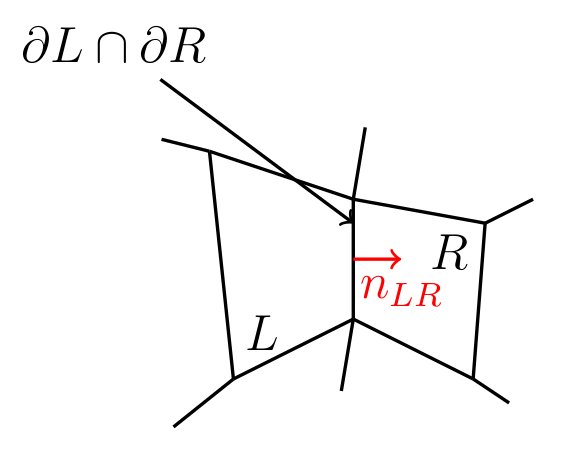
\includegraphics[width=8cm]{./cell_LR.png}
\caption{Maillage: conventions de notation.\label{fig:normal}}
\end{center}
\end{figure}

Théoriquement pour calculer $f^{n}$ à partir de $f^{n-1}$ en appliquant
le schéma DG (\ref{eq:dg_imp}) il faudrait résoudre un système linéaire
ce qui peut-être très coûteux en 3D. Heureusement en utilisant deux
propriétés du schéma DG: discontinuité de la solution numérique et
décentrage du flux, nous constatons qu'il est possible de résoudre
le système linéaire de proche en proche en parcourant le maillage
dans le sens de la vitesse $v$. Plus nous avançons dans le maillage,
plus le calcul devient parallèle.


\subsection{Graphe de dépendance}

Afin d'expliquer ce fait, nous considérons le maillage décrit dans
la figure \ref{fig:mesh-graph} où seules les macrocellules sont représentées.
Pour calculer $f^{n}$ dans la macrocellule 0, il suffit d'appliquer
les conditions aux limites. Ensuite, nous pouvons calculer en parallèle
les valeurs de $f^{n}$ dans les cellules 1 et 3 à partir des résultats
de la cellule 0, etc. Les dépendances des calculs peuvent être schématisées
par un graphe orienté également indiqué sur la figure \ref{fig:mesh-graph}.

\begin{center}
\begin{figure}
\begin{centering}
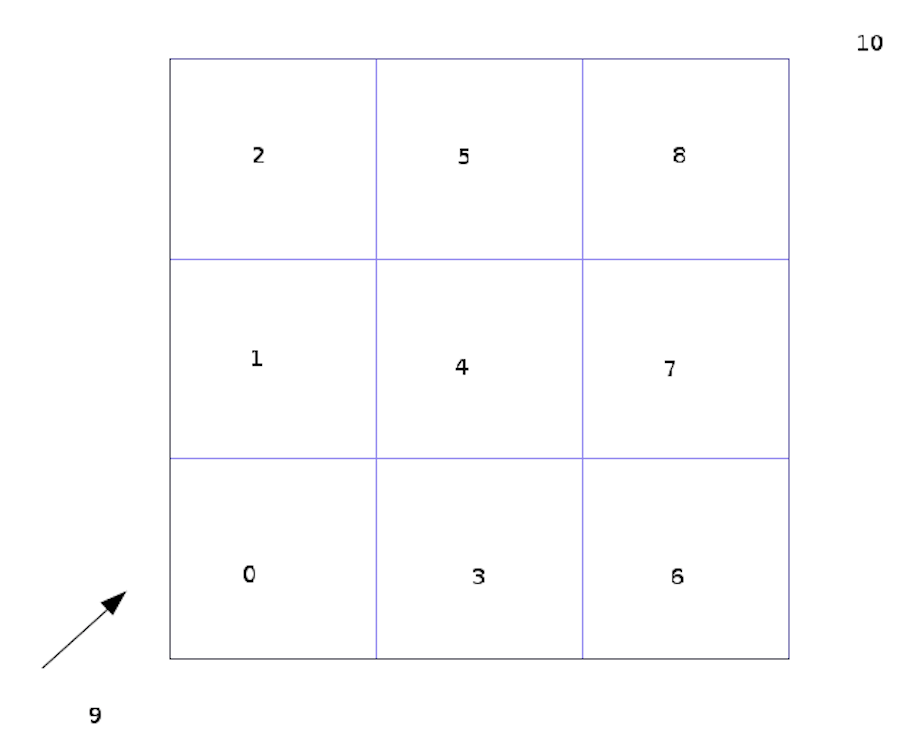
\includegraphics[width=8cm]{./cubegros.png}$\quad$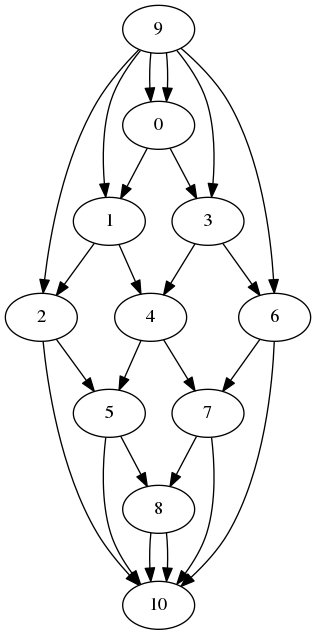
\includegraphics[height=8cm]{./upwindgraph.png}
\par\end{centering}

\caption{Parcourt d'un maillage dans le sens de la vitesse. À gauche: un exemple
de maillage et de vitesse. À droite: graphe de dépendance correspondant.
Cette construction se généralise à des maillages déstructurés.\label{fig:mesh-graph}}
\end{figure}

\par\end{center}

L'organisation des calculs et le parallélisme qui en découle sont très
naturels. Mais il est aussi délicat à programmer simplement et efficacement:
comment répartir les calculs sur les coeurs de calcul disponibles
?


\subsection{Implémentation StarPU}

StarPU permet de décrire de façon simple et effnnousicace ce type
d'algorithme. L'algorithme consiste d'abord à construire le graphe
de dépendance des macrocellules. Ensuite il faut effectuer un tri,
dit topologique, des nœuds du graphe. Ensuite, pour chaque macrocellule
parcourue dans l'ordre topologique, il faut:
\begin{itemize}
\item calculer les termes volumiques du schéma DG (\ref{eq:dg_imp});
\item calculer les flux amont des macrocellules précédemment calculées
ou venant des conditions aux limites;
\item résoudre un petit système linéaire local à la macrocellule;
\item extraire les données vers les macrocellules aval.
\end{itemize}
Chacune de ces étapes est décrite avec des tâches et des codelettes
StarPU. Ces tâches sont ensuite soumises dans un ordre correct au
support d'exécution, grâce à la numérotation topologique. C'est StarPU
qui se charge de la parallélisation et des transferts de données en
mémoire.


\subsection{Résultats}

Nous comparons le solveur linéaire direct du système complet avec
le solveur de proche en proche pour diverses tailles des macrocellules.
En effet, la gestion du graphe des tâches par StarPU a un coût. Il
faut donc soumettre des tâches suffisamment grosses pour que ce surcoût
soit amorti. Nous constatons dans nos expériences qu'il existe un
découpage optimal entre les macro et les sous-cellules pour lequel
le parallélisme de StarPU est très efficace. Les résultats sont alors
très proches du parallélisme optimal auquel on peut s'attendre pour
ce type d'algorithme de progression par front (sur un maillage $n\times n$,
au meilleur de la progression, il est possible de calculer en parallèle
$n$ macrocellules).

\begin{table}
\begin{centering}
\begin{tabular}{|c|c|c|c|c|c|c|}
\hline
nb cores & 0 & 1 & 2 & 4 & 8 & 16\tabularnewline
\hline
\hline
$10\times10\times8\times8$ direct & 30 & 144 & - & - & - & -\tabularnewline
\hline
$10\times10\times8\times8$ upwind & - & 32 & 19 & 12 & 7 & 6\tabularnewline
\hline
$20\times20\times4\times4$ upwind & - & 41 & 26 & 17 & 12 & 17\tabularnewline
\hline
$20\times20\times8\times8$ upwind & - & 120 & 72 & 40 & 28 & 20\tabularnewline
\hline
\end{tabular}
\par\end{centering}

\caption{Étude d'accélération StarPU pour le solveur frontal. AMD Opteron 16
cores, 2.8 Ghz. Temps en secondes secondes pour 200 iterations de
la méthode temporelle. En fonction du découpage des macrocellules,
le parallélisme est plus ou moins efficace.\label{tab:scaling-upwind}}
\end{table}


StarPU offre aussi la possibilité de visualiser le graphe des tâches.
Un exemple est donné figure \ref{fig:zoom-dag}. Il est aussi possible
de visualiser le diagramme de Gantt de l'ordonnancement des tâches.
Un tel diagramme est représenté Figure \ref{fig:gantt}. Nous y comparons
deux stratégies d'ordonnancement. Dans la première approche, nous
imposons un point de synchronisation à la fin de chaque pas de temps.
Nous voyons alors que la file d'attente se vide périodiquement. Dans
la seconde approche, nous n'imposons aucun point de synchronisation.
La file d'attente se remplit donc pendant une première phase, avant
de se vider dans la seconde partie du calcul. Cette deuxième approche
est légèrement plus efficace que la première (gain de l'ordre de 10\%).
Sans StarPU, tester la seconde approche n'aurait pas été aussi simple.

\begin{center}
\begin{figure}
\begin{centering}
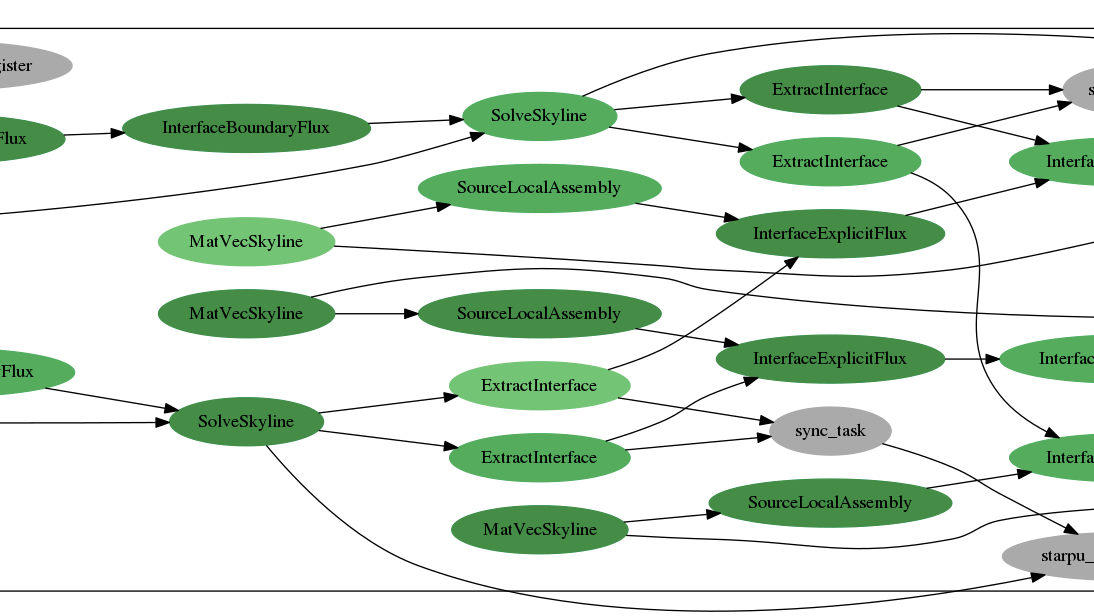
\includegraphics[height=8cm]{./zoom-dag.png}
\par\end{centering}

\caption{Zoom sur le graphe des ta\^{c}hes générés par StarPU\label{fig:zoom-dag}}
\end{figure}

\par\end{center}

\begin{center}
\begin{figure}
\begin{centering}
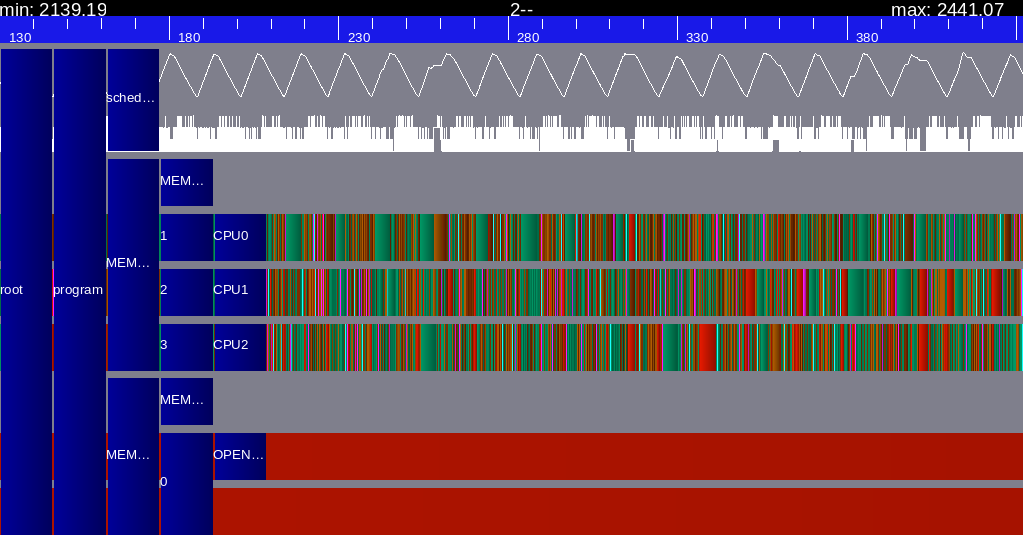
\includegraphics[height=8cm]{./withsync.png}
\par\end{centering}

\begin{centering}
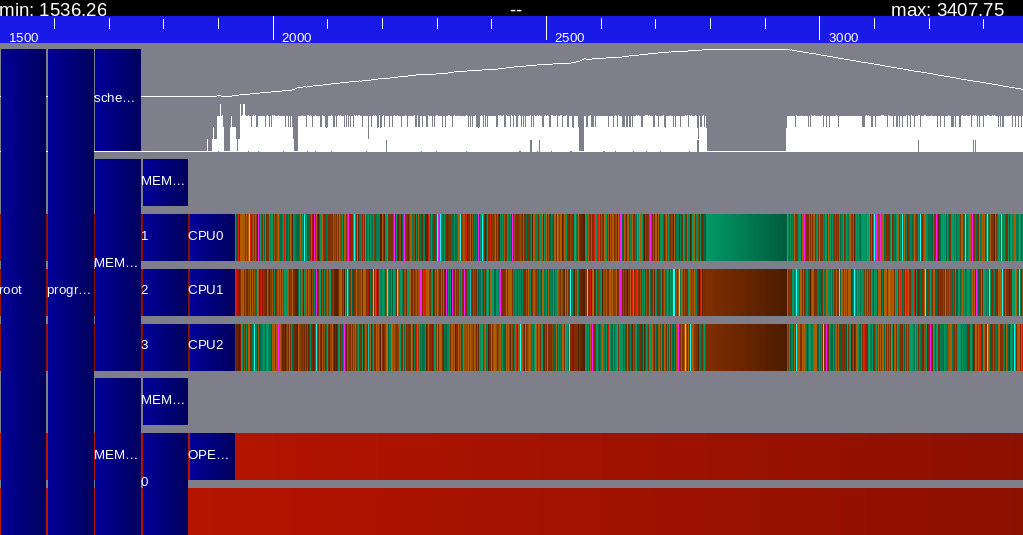
\includegraphics[height=8cm]{./nosync.png}
\par\end{centering}

\caption{Deux stratégies d'ordonnancement. Diagramme de Gantt généré par StarPU.
En haut: synchronisation à la fin de chaque pas de temps. En bas:
pas de synchronisation. \label{fig:gantt}}
\end{figure}

\par
\end{center}


\section{Application à DG explicite}


\subsection{Implémentation OpenMP}

Nous avons programmé une version C/OpenMP d'un code DG explicite sur
maillage structuré. Ce code a été optimisé à la fois en terme de parallélisme
(vectorisation des boucles) mais aussi en terme d'accès mémoire grâce
à une technique dite de tiling afin d'exploiter au mieux la mémoire
cache du CPU. Ces optimisations sont sans doute très proches du maximum
de ce qu'on peut obtenir avec un processeur multicore. Nous avons
été assistés dans ce travail par V. Loechner, collègue informaticien
à Strasbourg \cite{helluy2015asynchronous}.


\subsection{Implémentation StarPU}

Nous avons programmé dans SCHNAPS une version StarPU de l'algorithme
DG explicite. Pour cela, comme dans Teta, nous avons découpé le calcul
en tâches élémentaires et programmé les codelettes correspondantes.

Un gros avantage de la programmation StarPU par rapport à un code
purement OpenCLest que nous n'avons pas à expliciter à la main les
dépendances entre tâches. Il suffit de préciser quelles sont les données
en lecture (R), écriture (W) ou lecture-écriture (RW) de chaque tâche.
Par ailleurs la possibilité de tracer le graphe des tâches de StarPU
ainsi que des diagrammes de Gantt de l'ordonnancement est très utile
pour le débogage ou l'amélioration des performances.

Nous avons aussi pour chaque tâche programmé une codelette C pour
CPU et une codelette OpenCL pour GPU. Ainsi StarPU peut choisir à
l'exécution de lancer telle ou telle tâche sur CPU ou GPU. Nous avons
aussi pour certaines codelettes C écrit plusieurs versions.


\section{Résultats}


\subsection{Comparaison OpenMP/OpenCL}

Dans ce test, nous comparons le programme DG OpenMP avec une implémentation
OpenCL du même algorithme. L'avantage de la version OpenCL est qu'elle
peut être indifféremment être exécutée sur CPU ou GPU .Voir tableau
\ref{tab:openmp-opencl}.

\begin{table}

\begin{center}

  \begin{tabular}{|c|c|c|}     \hline     Implementation & Time & Speedup\tabularnewline     \hline     \hline     OpenMP (Intel CPU 12 cores) & 717 s & 1\tabularnewline     \hline     OpenCL (Intel CPU 12 cores) & 996 s & 0.7\tabularnewline     \hline     OpenCL (NVIDIA K20) & 45 s & 16\tabularnewline     \hline     OpenCL (AMD HD7970) & 38 s & 19\tabularnewline     \hline     OpenCL + MPI (4 x NVIDIA K20) & 12 s & 58\tabularnewline     \hline   \end{tabular}

\caption{Comparaison des différentes implémentations de la méthode DG sur une
grille régulière. Métériel : 2$\times$ Intel(R) Xeon(R) E5-2630 (6
cores, 2.3GHz), AMD Radeon HD 7970, NVidia K20m. Sur les CPU Intel
l'hyperthreading est désactivé.\label{tab:openmp-opencl} }

\end{center}

\end{table}
Dans ce tableau, nous constatons que l'implémentation OpenMP est la
plus efficace sur CPU. Cependant la version OpenCL n'est pas loin
derrière sur CPU avec une perte de seulement 30\%. Cette perte s'explique
par le fait que le code OpenCL a été optimisé pour GPU. Certains transferts
en mémoire cache sont inutiles dans le cas du CPU et ralentissent
les calculs sur ce type d'architecture.

Il est possible de spécialiser les kernels OpenCL et de choisir à
l'exécution la version la plus efficace selon que l'on est sur CPU
et GPU. Cette stratégie permettrait d'atteindre la même efficacité
avec le code OpenCL qu'avec le code OpenMP, y compris sur CPU. Une
étude en ce sens est proposée par exemple dans \cite{shen2012performance}.

Sur GPU l'accélération du code OpenCL est bien sûr très efficace.


\subsection{Comparaisons C/StarPU-C}

Afin d'évaluer les performances de l'implémentation StarPU pour le
schéma explicite, nous comparons un code C non optimisé avec le code
StarPU où seules les codelettes C sont autorisées. Ceci peut se faire
en positionnant la variable d'environnement STARPU\_NOPENCL à 0.

Le cas de calcul est celui d'une onde électromagnétique plane se propageant
dans un domaine de forme cylindrique. Le maillage est constitué de
40 macrocellules DG de degré 2. Nous comparons les
performances obtenues avec divers ordonnanceurs (``eager'' ou ``dmda'')
et pour diverses tailles du maillage ($2^3$ sous-cellules ou $3^3$ sous-cellules
par macrocellule).
Nous obtenons les résultats du tableau \ref{tab:spu-c}.

\begin{table}
\begin{tabular}{|c|c|c|c|c|c|c|}
\hline
nb cores & 1 (c) & 1 (spu) & 2 (spu) & 4 (spu) & 8 (spu) & speedup (c/spu)\tabularnewline
\hline
\hline
$2^3$, eager & 48 & 34 & 18 & 11 & 5 & 6.8 \tabularnewline
\hline
$2^3$, dmda & 48 & 32 & 20 & 12 & 6 &  5.3 \tabularnewline
\hline
$3^3$, eager & 214 & 187 & 109 & 59 & 23 & 8.1 \tabularnewline
\hline
$3^3$, dmda & 214 & 181 & 118 & 65 & 25 &  7.2 \tabularnewline
\hline
\end{tabular}

\caption{Comparaison des temps de calcul C/Starpu-C\label{tab:spu-c}}
\end{table}


StarPU permet d'étudier l'efficacité de l'ordonnanceur. On constate
par exemple sur la figure \ref{fig:gantt2cpu} que tous les ``workers''
StarPU (c'est à dire les coeurs de CPU) sont bien exploités: peu d'attentes
(représentées en rouge). Les transferts mémoires (flèches blanches) sont
également limités.

\begin{center}
\begin{figure}
\begin{centering}
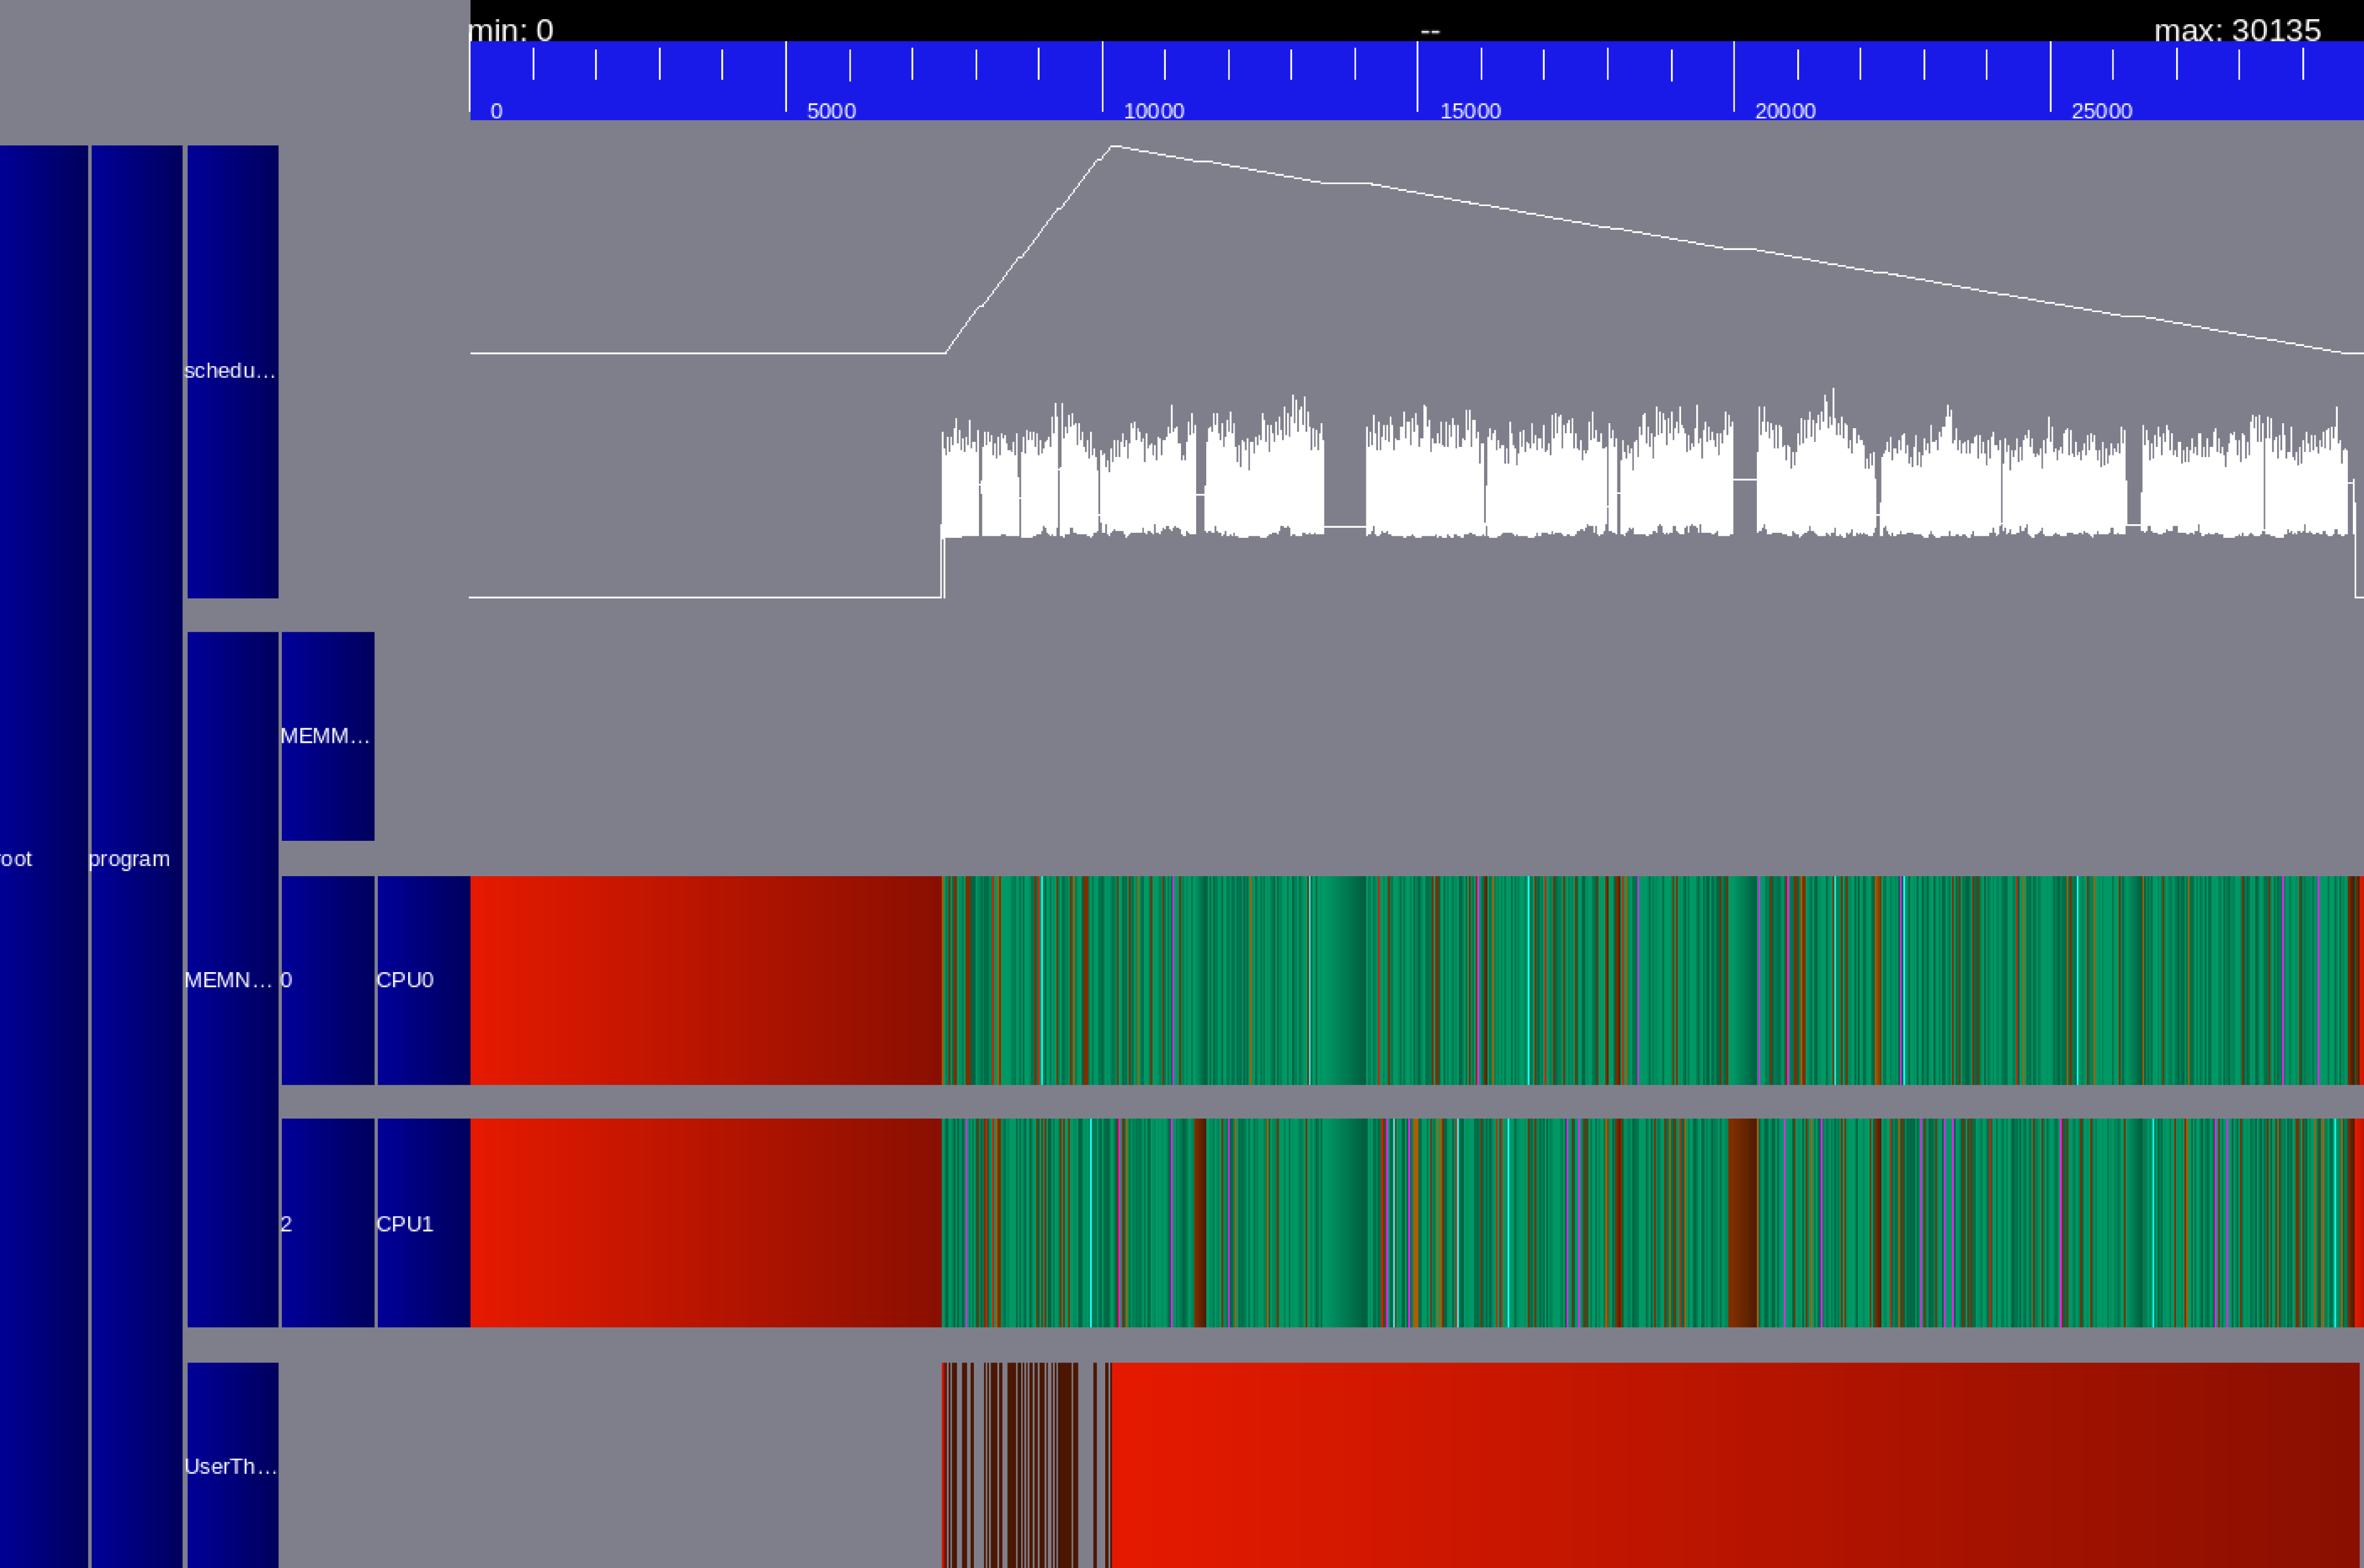
\includegraphics[height=8cm]{./gantt2cpu.png}
\par\end{centering}

\caption{Exécution en parallèle sur deux cœurs CPU. Diagramme de Gantt généré par StarPU.\label{fig:gantt2cpu}}
\end{figure}

\par\end{center}

\subsection{Comparaisons StarPU-C/StarPU-C+OpenCL}

Dans ce test on cherche à évaluer l'apport de l'activation des GPU
dans le calcul StarPU. Pour cela, on positionne la variable d'environnement
STARPU\_NOPENCL de 0 à 2 (nombre de GPU à activer). Le maillage est
fixé à une taille de 40 macrocellules DG découpées en $3^3$ sous-cellules. Les résultats sont présentés
dans le tableau \ref{tab:spu-c-opencl}.

\begin{table}
\begin{center}
\begin{tabular}{|c|c|c|c|c|}
\hline
 & 0 GPU & 1 GPU & 2 GPU & max. speedup \tabularnewline
\hline
\hline
C+OpenCL (eager) & 59 & 40 & 36 & 1.6 \tabularnewline
\hline
C+OpenCL (dmda) & 65 & 43 & 38 & 1.7 \tabularnewline
\hline
\end{tabular}

\caption{Comparaison des temps de calcul StarPU-C/StarPU-C+OpenCL\label{tab:spu-c-opencl}}
\end{center}
\end{table}
On constate que l'activation des GPU apporte une légère accélération.
Cependant, celle-ci est limitée, quelle que soit l'ordonnanceur. C'est
assez surprenant et décevant, car l'ordonnanceur ``dmda'' est sensé
tenir compte des transferts mémoire pour la distribution des tâches.
Notre découpage des données ne devrait impliquer des transferts qu'aux
interfaces entre les zones de calcul. Nous allons prendre contact
avec les développeurs StarPU pour mieux comprendre ce défaut de performance.
Nous avons soumis un projet de recherche au CEMRACS 2016 \url{http://smai.emath.fr/cemracs/cemracs16/}.
Il est prévu que nous rencontrions des experts de StarPU lors de ce
projet.



\section{Optimisations OpenCL CPU}

\subsection{Axes d'optimisation}

Le solveur Teta a initialement été programmé et optimisé pour être exécuté
sur GPU\footnote{T. Strub. 2015. Résolution des équations de Maxwell tridimensionnelles
instationnaires sur architecture massivement multicœur. Mémoire de thèse. 2015.}.
Les kernels OpenCL qu'il contient sont utilisables sur CPU mais ne
produisent pas de bons résultats en terme de performances. De manière générale,
un kernel OpenCL optimisé GPU ne sera pas efficace sur CPU. Plusieurs axes de
développement sont conseillés par les constructeurs de CPU (AMD, Intel), en voici
une liste non exhaustive :
\begin{itemize}
\item Favoriser la mémoire globale à la mémoire locale : généralement, la mémore locale
d'un CPU est globale ;
\item Augmenter la taille des work-groups (pour en diminuer le nombre) et sérialiser les
traitements au sein d'un kernel : les changements de work-groups sont coûteux en temps ;
\item Favoriser le stockage des données qui seront recalculées ;
\item Utiliser les unités de calcul vectoriel SSE ou AVX si disponibles.
\end{itemize}
Ces axes d'optimisation ont été explorés (en partie) dans le cadre du projet HOROCH et
nous verrons les gains obtenus dans la section suivante.

\subsection{Résultats}

Afin d'évaluer les performances suite à l'optimisation des kernels OpenCL pour CPU, nous
comparons les temps de chaque kernel d'une même simulation avant et après modifications.
Les résultats sont dépendants du matériel et ont été obtenus avec un CPU Intel Core i7-920
\@ 2,67 GHz et un GPU NVIDIA GeForce GTX 460. Avec cette configuration, le ratio de temps
CPU/GPU avant optimisations était de 18.

Seuls les kernels ``Volume'' et ``Surface'' qui représentent respectivement les flux intra
et inter éléments ont été modifié. Ces deux kernels représentaient 92\% du temps total avant
optimisations. Ils ont été modifié pour ne plus utiliser la mémoire locale,
pour qu'un work-item traite un élément complet / une surface complète et non plus un seul point
d'interpolation et pour que les données d'interpolation soient stockées à la première
itération puis réutilisées.

\begin{table}
\begin{center}
\begin{tabular}{|c|c|c|}
\hline
 & avant (\%) & après (\%)\tabularnewline
\hline
\hline
Volume & 48 & 13\tabularnewline
\hline
Surface & 49 & 71\tabularnewline
\hline
Mass & 2 & 10\tabularnewline
\hline
RK2 & 1 & 6\tabularnewline
\hline
\end{tabular}

\caption{Comparaison des ratios de temps entre les différents kernels avant et après
optimisations OpenCL CPU\label{tab:ocl_opti_cpu}}
\end{center}
\end{table}

Avec ces optimisations, le CPU a connu un speedup de 5,6 par rapport aux temps obtenus
avec les kernels optimisés GPU. Ce speedup ramène le ratio de temps CPU/GPU à 3,2. Le tableau
\ref{tab:ocl_opti_cpu} présente l'évolution des ratios de temps entre les différents kernels
avant et après modifications.

Suite aux adaptations effectuées dans les fonctions d'interpolation, le GPU a lui aussi connu
un impact positif avec un speedup de 1,4. Le ratio de temps CPU/GPU réel est donc de 4,5 en
comptant cet impact.



\section{Conclusion et perspectives}

En conclusion de cette tâche ``Parallélisation hybride'' nous sommes
arrivés aux conclusions suivantes:
\begin{itemize}
\item Pour des architectures de codes complexes, OpenMP et son système de
directives n'est pas forcément très indiqué pour réaliser des conceptions
parallèles efficaces.
\item L'écriture d'un code OpenCL est un peu plus compliquée, mais apporte
l'avantage énorme de pouvoir tourner à la fois sur CPU et GPU. Sur
CPU il est possible d'atteindre les mêmes performances qu'avec OpenMP.
\item Les outils récents de génération automatique de code parallèle (pocc,
PLUTO, DSL, etc.) sont très prometteurs, mais en l'état actuel de
la technologie, ils sont encore en phase de recherche et développement.
En général ils fonctionnent sur des codes simples ou des exemples
assez académiques. Il s'agit néanmoins d'un domaine en évolution très
rapide et il faut maintenir une veille technologique sur ces outils
(ce à quoi nous nous employons).
\item StarPU est le système de parallélisation par tâches le plus avancé
à l'heure actuelle. Il est d'emploi assez aisé, efficace. Les outils
annexes sont très utiles pour le débogage et l'optimisation.
\item Les performances de notre implémentation StarPU de l'alogirthmel'algorithme DG
sont cependant décevantes lorsque l'on mixe des CPU et des GPU. Ces
résultats, obtenus récemment, sont décevants et assez inexplicables
pour l'instant, car StarPU a justement été développé pour le calcul
hybride. Nous allons prendre contact cet été (2016) avec des développeurs
StarPU pour comprendre d'où provient ce défaut de performances.
\end{itemize}
\bibliographystyle{plain}
\bibliography{horoch_juin2016}

\end{document}
\grid
